\section{Multi-Graph Additions}
An additional contribution this work offers is the expansion to night vs day charging. Day and night operations differ in two aspects: number of chargers, and bus availability. During the day, the buses can charge on chargers in the charge station. The number of chargers in the station are limited, causing contention between buses. At night, each bus docks in a holding stall with one charger per stall, eliminating charger contention. 
\par Bus availability also changes because buses do not leave their stalls at night. This simplifies the charge problem because buses are always available for charging. 
\par Equation \ref{eqn:cFlow} in section \ref{sec:net-flow} describes the net-flow constraints which constrain the number of chargers in the source and sink nodes. Because the number of chargers are different from night to day, a separate graph is used at each transition as shown in figure \ref{fig:nightVsDayGraph}.
\par Each graph is connected by equating the appropriate SOC values.  Consider the multi-graph formulation given in figure \ref{fig:nightVsDayConnected}.  The morning graph is related to the day graph because $d_{1,1}$ and $d_{2,1}$ represent the same SOC values as $d_{1,2}$ and $d_{2,2}$ respectively. The same applies for the day and night graph, where $d_{1,5}$ and $d_{2,5}$ represent the SOC values for $d_{1,6}$ and $d_{2,6}$. This equality relationship can be expressed as an equality constraint where
\begin{align}
	\mathbf{d}_{\text{graph 1}} - \mathbf{d}_{\text{graph 2}} = \mathbf{0}
\end{align}
or by 
\begin{align}\label{eqn:multiGraphConst}
	D_\text{multi-graph}\mathbf{y} = \mathbf{0},
\end{align}
where $D_\text{multi-graph}$ is an $\text{nBus} \times \text{nVar}$ matrix such that
\begin{align}
	D_\text{multi-graph}\mathbf{y} = \mathbf{d}_{\text{graph 1}} - \mathbf{d}_{\text{graph 2}}.
\end{align}
Because all SOC values $d$ are contained in $\mathbf{y}$, forming the matrix $D$ amounts to placing $1$ and $-1$ at the indices corresponding to $d_{\text{graph 1}}$ and $d_{\text{graph 2}}$ respectively and zero otherwise. 
\begin{figure*}
	\centering
	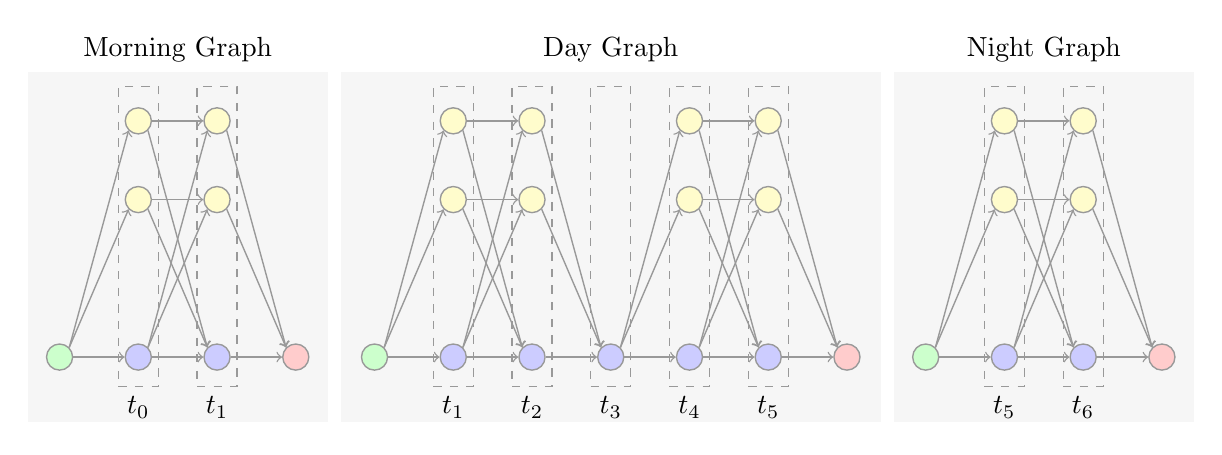
\begin{tikzpicture} 
		% morning graph
		\node[rectangle, fill=gray!7, minimum width=1.5in, minimum height=1.75in, label=above:Morning Graph](mBox) at (-2.5,1.4){};
		\node[rectangle, draw=black!40, dashed, minimum width=0.2in, minimum height = 1.5in, label=below:$t_0$](boxT0) at (-3,1.53){};
		\node[rectangle, draw=black!40, dashed, minimum width=0.2in, minimum height = 1.5in, label=below:$t_1$](boxT0) at (-2,1.53){};
		\node[circle, fill=green!20, line width=0.5pt, draw=black!40, minimum size=0.1in](mOne) at (-4,0){};
		\node[circle, fill=blue!20, line width=0.5pt, draw=black!40, minimum size=0.1in](mTwo) at (-3,0){}; 
		\node[circle, fill=blue!20, line width=0.5pt, draw=black!40, minimum size=0.1in](mThree) at (-2,0){};
		\node[circle, fill=red!20, line width=0.5pt, draw=black!40, minimum size=0.1in](mFour) at (-1,0){};

		\node[circle, fill=yellow!20, line width=0.5pt, draw=black!40, minimum size=0.1in](mFive) at (-3,2){};
		\node[circle, fill=yellow!20, line width=0.5pt, draw=black!40, minimum size=0.1in](mSix) at (-2,2){};
		\node[circle, fill=yellow!20, line width=0.5pt, draw=black!40, minimum size=0.1in](mSeven) at (-3,3){};
		\node[circle, fill=yellow!20, line width=0.5pt, draw=black!40, minimum size=0.1in](mEight) at (-2,3){};

		\draw[->, line width=0.5pt, color=black!40] (mOne.east) -- (mTwo.west){};
		\draw[->, line width=0.5pt, color=black!40] (mTwo.east) -- (mThree.west){};
		\draw[->, line width=0.5pt, color=black!40] (mThree.east) -- (mFour.west){};

		\draw[->, line width=0.5pt, color=black!40] (mOne.north east) -- (mFive.south west){};
		\draw[->, line width=0.5pt, color=black!40] (mTwo.north east) -- (mSix.south west){};
		\draw[->, line width=0.5pt, color=black!40] (mOne.north east) -- (mSeven.south west){};
                \draw[->, line width=0.5pt, color=black!40] (mTwo.north east) -- (mEight.south west){};

                \draw[->, line width=0.5pt, color=black!40] (mFive.south east) -- (mThree.north west){}; 
                \draw[->, line width=0.5pt, color=black!40] (mSix.south east) -- (mFour.north west){};
                \draw[->, line width=0.5pt, color=black!40] (mSeven.south east) -- (mThree.north west){};
		\draw[->, line width=0.5pt, color=black!40] (mEight.south east) -- (mFour.north west){};

                \draw[->, line width=0.5pt, color=black!40] (mFive.east) -- (mSix.west){};
                \draw[->, line width=0.5pt, color=black!40] (mSeven.east) -- (mEight.west){};

		% night graph
		\node[rectangle, fill=gray!7, minimum width=1.5in, minimum height=1.75in, label=above:Night Graph](nBox) at (8.5,1.4){};
		\node[rectangle, draw=black!40, dashed, minimum width=0.2in, minimum height = 1.5in, label=below:$t_6$](boxT2) at (9,1.53){};
		\node[rectangle, draw=black!40, dashed, minimum width=0.2in, minimum height = 1.5in, label=below:$t_5$](boxT0) at (8,1.53){};
		\node[circle, fill=green!20, line width=0.5pt, draw=black!40, minimum size=0.1in](nOne) at (7,0){};
		\node[circle, fill=blue!20, line width=0.5pt, draw=black!40, minimum size=0.1in](nTwo) at (8,0){}; 
		\node[circle, fill=blue!20, line width=0.5pt, draw=black!40, minimum size=0.1in](nThree) at (9,0){};
		\node[circle, fill=red!20, line width=0.5pt, draw=black!40, minimum size=0.1in](nFour) at (10,0){};

		\node[circle, fill=yellow!20, line width=0.5pt, draw=black!40, minimum size=0.1in](nFive) at (8,2){};
		\node[circle, fill=yellow!20, line width=0.5pt, draw=black!40, minimum size=0.1in](nSix) at (9,2){};
		\node[circle, fill=yellow!20, line width=0.5pt, draw=black!40, minimum size=0.1in](nSeven) at (8,3){};
		\node[circle, fill=yellow!20, line width=0.5pt, draw=black!40, minimum size=0.1in](nEight) at (9,3){};

		\draw[->, line width=0.5pt, color=black!40] (nOne.east) -- (nTwo.west){};
		\draw[->, line width=0.5pt, color=black!40] (nTwo.east) -- (nThree.west){};
		\draw[->, line width=0.5pt, color=black!40] (nThree.east) -- (nFour.west){};

		\draw[->, line width=0.5pt, color=black!40] (nOne.north east) -- (nFive.south west){};
		\draw[->, line width=0.5pt, color=black!40] (nTwo.north east) -- (nSix.south west){};
		\draw[->, line width=0.5pt, color=black!40] (nOne.north east) -- (nSeven.south west){};
                \draw[->, line width=0.5pt, color=black!40] (nTwo.north east) -- (nEight.south west){};

                \draw[->, line width=0.5pt, color=black!40] (nFive.south east) -- (nThree.north west){}; 
                \draw[->, line width=0.5pt, color=black!40] (nSix.south east) -- (nFour.north west){};
		\draw[->, line width=0.5pt, color=black!40] (nSeven.south east) -- (nThree.north west){};
		\draw[->, line width=0.5pt, color=black!40] (nEight.south east) -- (nFour.north west){};

		\draw[->, line width=0.5pt, color=black!40] (nFive.east) -- (nSix.west){};
                \draw[->, line width=0.5pt, color=black!40] (nSeven.east) -- (nEight.west){};


		% day graph	
		\node[rectangle, fill=gray!7, minimum width=2.7in, minimum height=1.75in, label=above:Day Graph](dBox) at (3,1.4){}; 
		\node[rectangle, draw=black!40, dashed, minimum width=0.2in, minimum height = 1.5in, label=below:$t_1$](boxT2) at (1,1.53){};
		\node[rectangle, draw=black!40, dashed, minimum width=0.2in, minimum height = 1.5in, label=below:$t_2$](boxT2) at (2,1.53){};
		\node[rectangle, draw=black!40, dashed, minimum width=0.2in, minimum height = 1.5in, label=below:$t_3$](boxT0) at (3,1.53){};
		\node[rectangle, draw=black!40, dashed, minimum width=0.2in, minimum height = 1.5in, label=below:$t_4$](boxT0) at (4,1.53){};
		\node[rectangle, draw=black!40, dashed, minimum width=0.2in, minimum height = 1.5in, label=below:$t_5$](boxT0) at (5,1.53){};
		\node[circle, fill=green!20, line width=0.5pt, draw=black!40, minimum size=0.1in](one) at (0,0){};
		\node[circle, fill=blue!20, line width=0.5pt, draw=black!40, minimum size=0.1in](two) at (1,0){}; 
		\node[circle, fill=blue!20, line width=0.5pt, draw=black!40, minimum size=0.1in](three) at (2,0){};
		\node[circle, fill=blue!20, line width=0.5pt, draw=black!40, minimum size=0.1in](four) at (3,0){};
		\node[circle, fill=blue!20, line width=0.5pt, draw=black!40, minimum size=0.1in](five) at (4,0){};
		\node[circle, fill=blue!20, line width=0.5pt, draw=black!40, minimum size=0.1in](six) at (5,0){};
		\node[circle, fill=red!20, line width=0.5pt, draw=black!40, minimum size=0.1in](seven) at (6,0){};
		
		\node[circle, fill=yellow!20, line width=0.5pt, draw=black!40, minimum size=0.1in](eight) at (1,2){};
		\node[circle, fill=yellow!20, line width=0.5pt, draw=black!40, minimum size=0.1in](nine) at (2,2){};
		\node[circle, fill=yellow!20, line width=0.5pt, draw=black!40, minimum size=0.1in](ten) at (4,2){};
		\node[circle, fill=yellow!20, line width=0.5pt, draw=black!40, minimum size=0.1in](eleven) at (5,2){};

		\node[circle, fill=yellow!20, line width=0.5pt, draw=black!40, minimum size=0.1in](twelve) at (1,3){};
		\node[circle, fill=yellow!20, line width=0.5pt, draw=black!40, minimum size=0.1in](thirteen) at (2,3){};
		\node[circle, fill=yellow!20, line width=0.5pt, draw=black!40, minimum size=0.1in](fourteen) at (4,3){};
		\node[circle, fill=yellow!20, line width=0.5pt, draw=black!40, minimum size=0.1in](fifteen) at (5,3){};

		\draw [->, line width=0.5pt, color=black!40] (one.east) -- (two.west);
		\draw [->, line width=0.5pt, color=black!40] (two.east) -- (three.west);
		\draw [->, line width=0.5pt, color=black!40] (three.east) -- (four.west);
		\draw [->, line width=0.5pt, color=black!40] (four.east) -- (five.west);
		\draw [->, line width=0.5pt, color=black!40] (five.east) -- (six.west);
		\draw [->, line width=0.5pt, color=black!40] (six.east) -- (seven.west);

		\draw [->, line width=0.5pt, color=black!40] (one.north east) -- (eight.south west);
		\draw [->, line width=0.5pt, color=black!40] (two.north east) -- (nine.south west);
		\draw [->, line width=0.5pt, color=black!40] (four.north east) -- (ten.south west);
		\draw [->, line width=0.5pt, color=black!40] (five.north east) -- (eleven.south west);
		\draw [->, line width=0.5pt, color=black!40] (eight.south east) -- (three.north west);
		\draw [->, line width=0.5pt, color=black!40] (nine.south east) -- (four.north west);
		\draw [->, line width=0.5pt, color=black!40] (ten.south east) -- (six.north west);
		\draw [->, line width=0.5pt, color=black!40] (eleven.south east) -- (seven.north west);
		\draw [->, line width=0.5pt, color=black!40] (eight.east) -- (nine.west);
		\draw [->, line width=0.5pt, color=black!40] (ten.east) -- (eleven.west); 

		\draw [->, line width=0.5pt, color=black!40] (one.north east) -- (twelve.south west);
		\draw [->, line width=0.5pt, color=black!40] (two.north east) -- (thirteen.south west);
		\draw [->, line width=0.5pt, color=black!40] (four.north east) -- (fourteen.south west);
		\draw [->, line width=0.5pt, color=black!40] (five.north east) -- (fifteen.south west);
		\draw [->, line width=0.5pt, color=black!40] (twelve.south east) -- (three.north west);
		\draw [->, line width=0.5pt, color=black!40] (thirteen.south east) -- (four.north west);
		\draw [->, line width=0.5pt, color=black!40] (fourteen.south east) -- (six.north west);
		\draw [->, line width=0.5pt, color=black!40] (fifteen.south east) -- (seven.north west);
		\draw [->, line width=0.5pt, color=black!40] (twelve.east) -- (thirteen.west);
		\draw [->, line width=0.5pt, color=black!40] (fourteen.east) -- (fifteen.west); 
	\end{tikzpicture}
	\caption{Night and Day Graphs}
	\label{fig:nightVsDayGraph}
\end{figure*}


\begin{figure*}
	\centering
	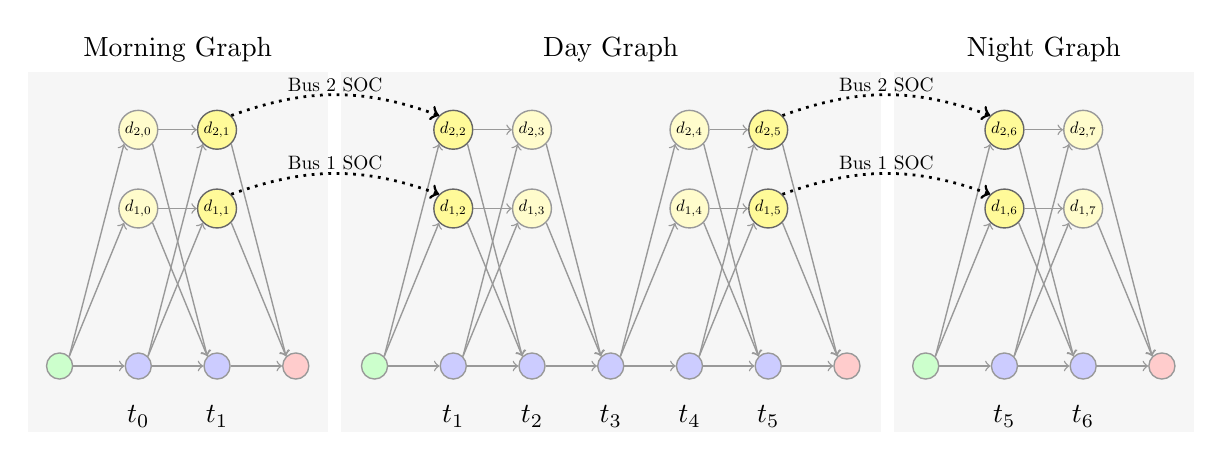
\begin{tikzpicture} 
		% morning graph
		\node[rectangle, fill=gray!7, minimum width=1.5in, minimum height=1.8in, label=above:Morning Graph](mBox) at (-2.5,1.45){};
		\node[rectangle, minimum width=0.2in, minimum height = 1.5in, label=below:$t_0$](boxT0) at (-3,1.53){};
		\node[rectangle, minimum width=0.2in, minimum height = 1.5in, label=below:$t_1$](boxT0) at (-2,1.53){};
		\node[circle, fill=green!20, line width=0.5pt, draw=black!40, minimum size=0.1in](mOne) at (-4,0){};
		\node[circle, fill=blue!20, line width=0.5pt, draw=black!40, minimum size=0.1in](mTwo) at (-3,0){};
		\node[circle, fill=blue!20, line width=0.5pt, draw=black!40, minimum size=0.1in](mThree) at (-2,0){};
		\node[circle, fill=red!20, line width=0.5pt, draw=black!40, minimum size=0.1in](mFour) at (-1,0){};

		\node[circle, fill=yellow!20, line width=0.5pt, draw=black!40, minimum size=0.1in, inner sep=1pt](mFive) at (-3,2){\scalebox{0.6}{$d_{1,0}$}};
		\node[circle, fill=yellow!40, line width=0.5pt, draw=black!60, minimum size=0.1in, inner sep=1pt](mSix) at (-2,2){\scalebox{0.6}{$d_{1,1}$}};
		\node[circle, fill=yellow!20, line width=0.5pt, draw=black!40, minimum size=0.1in, inner sep=1pt](mSeven) at (-3,3){\scalebox{0.6}{$d_{2,0}$}};
		\node[circle, fill=yellow!40, line width=0.5pt, draw=black!60, minimum size=0.1in, inner sep=1pt](mEight) at (-2,3){\scalebox{0.6}{$d_{2,1}$}};

		\draw[->, line width=0.5pt, color=black!40] (mOne.east) -- (mTwo.west){};
		\draw[->, line width=0.5pt, color=black!40] (mTwo.east) -- (mThree.west){};
		\draw[->, line width=0.5pt, color=black!40] (mThree.east) -- (mFour.west){};

		\draw[->, line width=0.5pt, color=black!40] (mOne.north east) -- (mFive.south west){};
		\draw[->, line width=0.5pt, color=black!40] (mTwo.north east) -- (mSix.south west){};
		\draw[->, line width=0.5pt, color=black!40] (mOne.north east) -- (mSeven.south west){};
                \draw[->, line width=0.5pt, color=black!40] (mTwo.north east) -- (mEight.south west){};

                \draw[->, line width=0.5pt, color=black!40] (mFive.south east) -- (mThree.north west){}; 
                \draw[->, line width=0.5pt, color=black!40] (mSix.south east) -- (mFour.north west){};
                \draw[->, line width=0.5pt, color=black!40] (mSeven.south east) -- (mThree.north west){};
		\draw[->, line width=0.5pt, color=black!40] (mEight.south east) -- (mFour.north west){};

                \draw[->, line width=0.5pt, color=black!40] (mFive.east) -- (mSix.west){};
                \draw[->, line width=0.5pt, color=black!40] (mSeven.east) -- (mEight.west){};

		% night graph
		\node[rectangle, fill=gray!7, minimum width=1.5in, minimum height=1.8in, label=above:Night Graph](nBox) at (8.5,1.45){};
		\node[rectangle, minimum width=0.2in, minimum height = 1.5in, label=below:$t_6$](boxT2) at (9,1.53){};
		\node[rectangle, minimum width=0.2in, minimum height = 1.5in, label=below:$t_5$](boxT0) at (8,1.53){};
		\node[circle, fill=green!20, line width=0.5pt, draw=black!40, minimum size=0.1in](nOne) at (7,0){};
		\node[circle, fill=blue!20, line width=0.5pt, draw=black!40, minimum size=0.1in](nTwo) at (8,0){}; 
		\node[circle, fill=blue!20, line width=0.5pt, draw=black!40, minimum size=0.1in](nThree) at (9,0){};
		\node[circle, fill=red!20, line width=0.5pt, draw=black!40, minimum size=0.1in](nFour) at (10,0){};

		\node[circle, fill=yellow!40, line width=0.5pt, draw=black!60, minimum size=0.1in, inner sep=1pt](nFive) at (8,2){\scalebox{0.6}{$d_{1,6}$}};
		\node[circle, fill=yellow!20, line width=0.5pt, draw=black!40, minimum size=0.1in, inner sep=1pt](nSix) at (9,2){\scalebox{0.6}{$d_{1,7}$}};
		\node[circle, fill=yellow!40, line width=0.5pt, draw=black!60, minimum size=0.1in, inner sep=1pt](nSeven) at (8,3){\scalebox{0.6}{$d_{2,6}$}};
		\node[circle, fill=yellow!20, line width=0.5pt, draw=black!40, minimum size=0.1in, inner sep=1pt](nEight) at (9,3){\scalebox{0.6}{$d_{2,7}$}};

		\draw[->, line width=0.5pt, color=black!40] (nOne.east) -- (nTwo.west){};
		\draw[->, line width=0.5pt, color=black!40] (nTwo.east) -- (nThree.west){};
		\draw[->, line width=0.5pt, color=black!40] (nThree.east) -- (nFour.west){};

		\draw[->, line width=0.5pt, color=black!40] (nOne.north east) -- (nFive.south west){};
		\draw[->, line width=0.5pt, color=black!40] (nTwo.north east) -- (nSix.south west){};
		\draw[->, line width=0.5pt, color=black!40] (nOne.north east) -- (nSeven.south west){};
                \draw[->, line width=0.5pt, color=black!40] (nTwo.north east) -- (nEight.south west){};

                \draw[->, line width=0.5pt, color=black!40] (nFive.south east) -- (nThree.north west){}; 
                \draw[->, line width=0.5pt, color=black!40] (nSix.south east) -- (nFour.north west){};
		\draw[->, line width=0.5pt, color=black!40] (nSeven.south east) -- (nThree.north west){};
		\draw[->, line width=0.5pt, color=black!40] (nEight.south east) -- (nFour.north west){};

		\draw[->, line width=0.5pt, color=black!40] (nFive.east) -- (nSix.west){};
                \draw[->, line width=0.5pt, color=black!40] (nSeven.east) -- (nEight.west){};


		% day graph	
		\node[rectangle, fill=gray!7, minimum width=2.7in, minimum height=1.8in, label=above:Day Graph](dBox) at (3,1.45){}; 
		\node[rectangle, minimum width=0.2in, minimum height = 1.5in, label=below:$t_1$](boxT2) at (1,1.53){};
		\node[rectangle, minimum width=0.2in, minimum height = 1.5in, label=below:$t_2$](boxT2) at (2,1.53){};
		\node[rectangle, minimum width=0.2in, minimum height = 1.5in, label=below:$t_3$](boxT0) at (3,1.53){};
		\node[rectangle, minimum width=0.2in, minimum height = 1.5in, label=below:$t_4$](boxT0) at (4,1.53){};
		\node[rectangle, minimum width=0.2in, minimum height = 1.5in, label=below:$t_5$](boxT0) at (5,1.53){};
		\node[circle, fill=green!20, line width=0.5pt, draw=black!40, minimum size=0.1in](one) at (0,0){};
		\node[circle, fill=blue!20, line width=0.5pt, draw=black!40, minimum size=0.1in](two) at (1,0){}; 
		\node[circle, fill=blue!20, line width=0.5pt, draw=black!40, minimum size=0.1in](three) at (2,0){};
		\node[circle, fill=blue!20, line width=0.5pt, draw=black!40, minimum size=0.1in](four) at (3,0){};
		\node[circle, fill=blue!20, line width=0.5pt, draw=black!40, minimum size=0.1in](five) at (4,0){};
		\node[circle, fill=blue!20, line width=0.5pt, draw=black!40, minimum size=0.1in](six) at (5,0){};
		\node[circle, fill=red!20, line width=0.5pt, draw=black!40, minimum size=0.1in](seven) at (6,0){};
		
		\node[circle, fill=yellow!40, line width=0.5pt, draw=black!60, minimum size=0.1in, inner sep=1pt](eight) at (1,2){\scalebox{0.6}{$d_{1,2}$}};
		\node[circle, fill=yellow!20, line width=0.5pt, draw=black!40, minimum size=0.1in, inner sep=1pt](nine) at (2,2){\scalebox{0.6}{$d_{1,3}$}};
		\node[circle, fill=yellow!20, line width=0.5pt, draw=black!40, minimum size=0.1in, inner sep=1pt](ten) at (4,2){\scalebox{0.6}{$d_{1,4}$}};
		\node[circle, fill=yellow!40, line width=0.5pt, draw=black!60, minimum size=0.1in, inner sep=1pt](eleven) at (5,2){\scalebox{0.6}{$d_{1,5}$}};

		\node[circle, fill=yellow!40, line width=0.5pt, draw=black!60, minimum size=0.1in, inner sep=1pt](twelve) at (1,3){\scalebox{0.6}{$d_{2,2}$}};
		\node[circle, fill=yellow!20, line width=0.5pt, draw=black!40, minimum size=0.1in, inner sep=1pt](thirteen) at (2,3){\scalebox{0.6}{$d_{2,3}$}};
		\node[circle, fill=yellow!20, line width=0.5pt, draw=black!40, minimum size=0.1in, inner sep=1pt](fourteen) at (4,3){\scalebox{0.6}{$d_{2,4}$}};
		\node[circle, fill=yellow!40, line width=0.5pt, draw=black!60, minimum size=0.1in, inner sep=1pt](fifteen) at (5,3){\scalebox{0.6}{$d_{2,5}$}};

		\draw [->, line width=0.5pt, color=black!40] (one.east) -- (two.west);
		\draw [->, line width=0.5pt, color=black!40] (two.east) -- (three.west);
		\draw [->, line width=0.5pt, color=black!40] (three.east) -- (four.west);
		\draw [->, line width=0.5pt, color=black!40] (four.east) -- (five.west);
		\draw [->, line width=0.5pt, color=black!40] (five.east) -- (six.west);
		\draw [->, line width=0.5pt, color=black!40] (six.east) -- (seven.west);

		\draw [->, line width=0.5pt, color=black!40] (one.north east) -- (eight.south west);
		\draw [->, line width=0.5pt, color=black!40] (two.north east) -- (nine.south west);
		\draw [->, line width=0.5pt, color=black!40] (four.north east) -- (ten.south west);
		\draw [->, line width=0.5pt, color=black!40] (five.north east) -- (eleven.south west);
		\draw [->, line width=0.5pt, color=black!40] (eight.south east) -- (three.north west);
		\draw [->, line width=0.5pt, color=black!40] (nine.south east) -- (four.north west);
		\draw [->, line width=0.5pt, color=black!40] (ten.south east) -- (six.north west);
		\draw [->, line width=0.5pt, color=black!40] (eleven.south east) -- (seven.north west);
		\draw [->, line width=0.5pt, color=black!40] (eight.east) -- (nine.west);
		\draw [->, line width=0.5pt, color=black!40] (ten.east) -- (eleven.west); 

		\draw [->, line width=0.5pt, color=black!40] (one.north east) -- (twelve.south west);
		\draw [->, line width=0.5pt, color=black!40] (two.north east) -- (thirteen.south west);
		\draw [->, line width=0.5pt, color=black!40] (four.north east) -- (fourteen.south west);
		\draw [->, line width=0.5pt, color=black!40] (five.north east) -- (fifteen.south west);
		\draw [->, line width=0.5pt, color=black!40] (twelve.south east) -- (three.north west);
		\draw [->, line width=0.5pt, color=black!40] (thirteen.south east) -- (four.north west);
		\draw [->, line width=0.5pt, color=black!40] (fourteen.south east) -- (six.north west);
		\draw [->, line width=0.5pt, color=black!40] (fifteen.south east) -- (seven.north west);
		\draw [->, line width=0.5pt, color=black!40] (twelve.east) -- (thirteen.west);
		\draw [->, line width=0.5pt, color=black!40] (fourteen.east) -- (fifteen.west); 


		\draw [dotted, color=black,-,line width=1pt] (mSix.north east) edge[->,bend left=20pt]node[above=-2.5pt]{\scalebox{0.7}{Bus 1 SOC}}(eight.north west); 
		\draw [dotted, color=black,-,line width=1pt] (mEight.north east) edge[->,bend left=20pt]node[above=-2.5pt]{\scalebox{0.7}{Bus 2 SOC}}(twelve.north west);

		\draw [dotted, color=black,-,line width=1pt] (eleven.north east) edge[->,bend left=20pt]node[above=-2.5pt]{\scalebox{0.7}{Bus 1 SOC}}(nFive.north west); 
		\draw [dotted, color=black,-,line width=1pt] (fifteen.north east) edge[->,bend left=20pt]node[above=-2.5pt]{\scalebox{0.7}{Bus 2 SOC}}(nSeven.north west);
	\end{tikzpicture}
	\caption{Bus SOC between Night and Day Graphs}
	\label{fig:nightVsDayConnected}
\end{figure*}
